%%%%%%%%%%%%%%%%%%%%%%%%%%%%%%%%%%%%%%%%%%%%%%%%%%%%%%%%%%%%%%%%%%%%%%%%%%%
% CHEP 2026 proceedings -- CernVM-FS Filebundles
% EPJ Web of Conferences (Web of Conferences LaTeX template)
%%%%%%%%%%%%%%%%%%%%%%%%%%%%%%%%%%%%%%%%%%%%%%%%%%%%%%%%%%%%%%%%%%%%%%%%%%%

\documentclass{webofc}
\usepackage[varg]{txfonts}   % Web of Conferences font
\usepackage{hyperref}
\usepackage{url}
\usepackage{listings}
\hypersetup{colorlinks=true,citecolor=blue,urlcolor=blue,linkcolor=blue}

% Compact listing style for the JSON bundle example
\lstdefinestyle{bundle}{
  basicstyle=\ttfamily\footnotesize,
  breaklines=true,
  columns=fullflexible,
  frame=single,
  framesep=4pt,
  xleftmargin=4pt,
  showstringspaces=false,
}

\begin{document}

\title{CernVM-FS Filebundles for low-latency software distribution
in interactive use cases}

\author{%
  \firstname{Valentin} \lastname{Volkl}\inst{1}\fnsep\thanks{\email{valentin.volkl@cern.ch}} \and
  \firstname{Georgios} \lastname{Christodoulis}\inst{1} \and
  \firstname{Jakob} \lastname{Blomer}\inst{1}
}

\institute{CERN, 1211 Geneva 23, Switzerland}

\abstract{%
CernVM-FS is a read-only, on-demand file system used to distribute
scientific software to the Worldwide LHC Computing Grid and many
communities beyond high-energy physics. Its lazy, per-file fetching is
highly efficient for batch computing, but it adds noticeable latency to
interactive sessions: starting an application that opens hundreds of
small files on a cold cache serializes one network round trip after
another. We present \emph{filebundles}, a mechanism that exploits the
predictable file-access pattern at application startup. A small bundle
specification, published next to a trigger file, declares the set of
files needed immediately after the trigger is opened. When a client
opens the trigger, CernVM-FS prefetches the listed dependencies
concurrently using a pool of worker threads, replacing a long serial
chain of requests with a short parallel prefetch phase. On a ROOT
startup benchmark, filebundles match local-disk performance and keep
startup time nearly flat as network latency grows, where the on-demand
baseline degrades linearly. The feature is available in CernVM-FS 2.14.
}

\maketitle

%======================================================================
\section{Introduction}
\label{sec-intro}

CernVM-FS~\cite{ref-cvmfs} is a global, read-only file system for the
distribution of scientific software. Rather than downloading and
unpacking a full software stack in advance, clients access it directly
from a globally available namespace under \texttt{/cvmfs}. Files are
fetched only when they are actually opened; downloading, decompression
and caching all happen transparently. For the user this resembles a
streaming service for scientific software: usage can start immediately,
and only the parts that are needed are ever transferred.

CernVM-FS is a core component of the Worldwide LHC Computing Grid, but
it is also widely used beyond high-energy physics, for example by
Euclid, LIGO, LSST, SKA and EESSI. The infrastructure spans on the
order of fifteen Stratum~1 mirror servers across Europe, the Americas
and Asia. Through \texttt{/cvmfs}, clients can access on the order of
$3.3\times10^{10}$ files and roughly 2~PB of data, with proven scaling
to much larger installations, and more than 8000 container images are
served, with the number of repositories continuing to grow.

This lazy, content-addressed model is extremely effective for
distributed batch computing, where the benefits of a shared software
distribution system dominate any per-file overhead. In interactive
sessions, however, the same on-demand behaviour can make application
startup noticeably slower than from local disk. This paper presents
\emph{filebundles}, a mechanism that reduces that startup latency by
prefetching the files an application needs immediately after launch.

%======================================================================
\section{Motivation}
\label{sec-motivation}

At the CernVM Users Workshop in 2022, Chris Burr (LHCb) highlighted a
practical limitation: in interactive sessions, CernVM-FS can be roughly
three to five times slower than local disk, even with a hot cache. For
distributed batch computing this is not a real concern, but in
interactive work startup latency matters: if opening an analysis
environment takes too long, the user experience suffers.

The effect is easy to reproduce on a controlled testbed. Installing
ROOT from a release tarball on local disk, importing ROOT in Python
takes about 2.47~s. Using the same software stack from \texttt{/cvmfs}
with a cold cache, the time increases to about 4.69~s. In this setup
the network path is very short, so the slowdown is not primarily a
bandwidth problem. It confirms that a significant part of the delay
comes from the way CernVM-FS serves many files on demand.

\subsection{Where does the time go?}
\label{sec-time}

When an application such as ROOT starts, it opens many files one after
another. On a cold cache, for each file CernVM-FS handles a FUSE
upcall, issues an HTTP request, waits for the round trip, downloads the
object, decompresses it and returns the data. This per-file overhead is
paid again and again, and because the requests are dependent they are
effectively serialized. The total amount of work is unremarkable, but
the serialized per-file latency adds up. In batch computing this
trade-off is acceptable; in interactive use the serialization is
precisely what hurts.

It is useful to recall the CernVM-FS cache hierarchy
(Fig.~\ref{fig-hierarchy}) in which any optimization has to operate. At
the top is the Stratum~0, the writable origin managed by the
repository maintainer (``librarian''). Below it are the globally
distributed Stratum~1 read-only mirrors. Sites typically add a Squid
forward proxy to absorb repeated requests from many clients. On each
worker node or workstation CernVM-FS keeps a local disk cache, and
above that the Linux kernel maintains the page cache. Filebundles
operate within this existing hierarchy. They do not change the data
model; they only change \emph{when} and \emph{how} the first wave of
file requests is issued.

\begin{figure}[t]
\centering
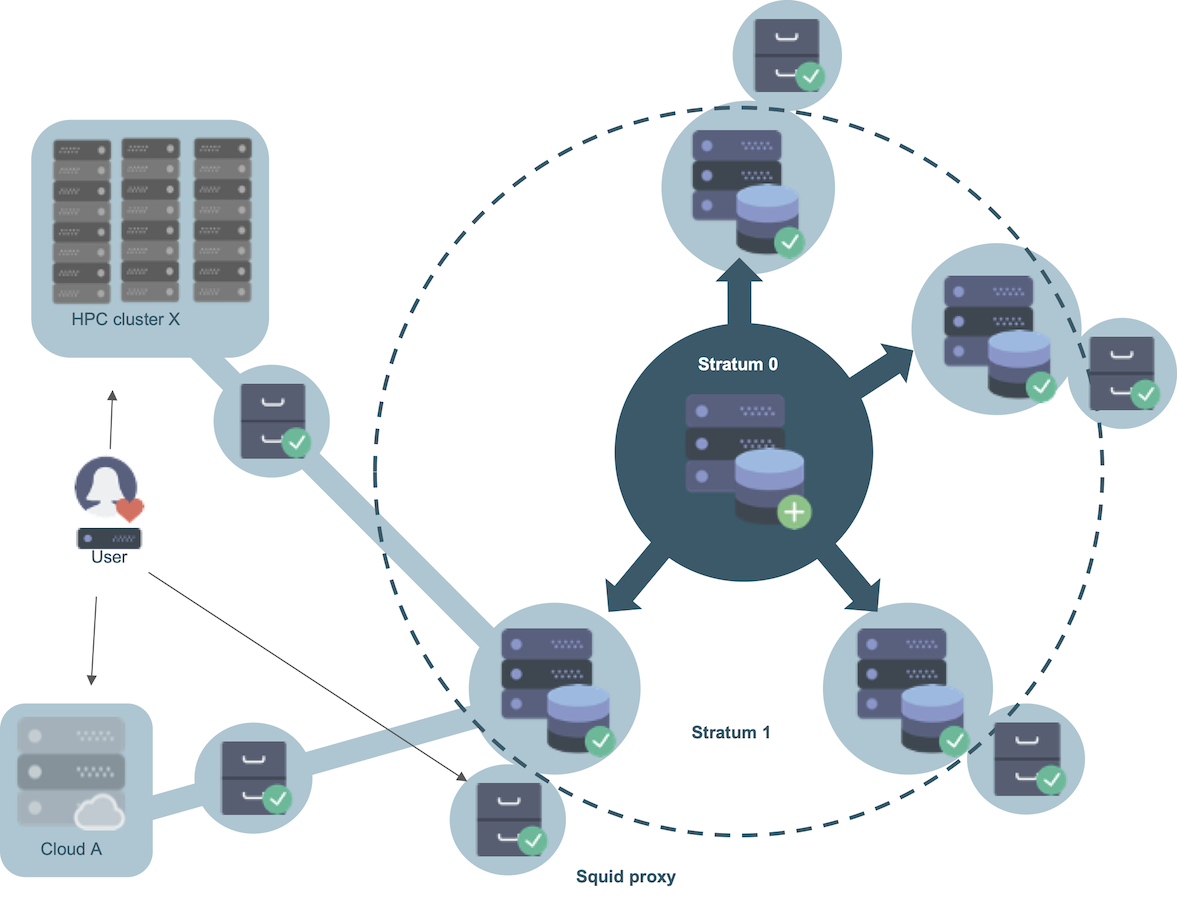
\includegraphics[width=0.78\textwidth]{figures/cvmfs_hierarchy.png}
\caption{The CernVM-FS cache hierarchy: a writable Stratum~0 origin,
globally distributed Stratum~1 mirrors, site-level Squid proxies, and
per-client disk and kernel page caches. Filebundles change only the
timing of the first wave of requests, not the data model.}
\label{fig-hierarchy}
\end{figure}

%======================================================================
\section{Filebundles}
\label{sec-design}

The central idea of filebundles is to exploit information we already
have about startup behaviour. For applications like ROOT or Python, the
set of files needed immediately after opening a given \emph{trigger}
file is often fairly predictable. Instead of discovering those
dependencies one file at a time, we describe them in advance.

A bundle is declared by a specification file published next to its
trigger file in the same directory, named
\texttt{.cvmfsbundle-<filename>}, where \texttt{<filename>} is the
trigger. The specification is a small, versioned JSON document holding
minimal metadata and a flat list of dependency paths, expressed as
absolute paths from the repository root. A representative ROOT bundle,
keyed on the Python package \texttt{\_\_init\_\_.py}, contains roughly
250 paths:

\begin{lstlisting}[style=bundle]
#%CVMFS_BUNDLE version=1 encoding=UTF-8
{
  "name": "CVMFS_BUNDLE",
  "version": "1.0.0",
  "encoding": "UTF-8",
  "dependencies": [
    "/root/lib/libCore.so",
    "/root/lib/libRIO.so",
    "/root/lib/libcppyy.so",
    "/root/lib/ROOT/_application.py",
    ...  (~250 paths total)
  ]
}
\end{lstlisting}

When a client opens the trigger file, CernVM-FS detects the matching
\texttt{.cvmfsbundle} specification and begins prefetching the listed
dependencies concurrently, using a pool of worker threads, while the
application continues to run. In effect, a long serial chain of
dependent requests is replaced by a much shorter parallel prefetch
phase that warms the local cache ahead of the application's subsequent
\texttt{open()} calls.

The feature is disabled by default and is enabled per mount through the
client configuration option \texttt{CVMFS\_PREFETCH\_FILEBUNDLES=yes}.
The decision whether bundle prefetching is active is taken once at
mount time, so clients that leave the option disabled incur no
additional overhead. The size of the prefetch thread pool is controlled
through \texttt{CVMFS\_BUNDLE\_POOL\_SIZE}.

\subsection{Publishing a filebundle}
\label{sec-publish}

From the librarian's point of view the workflow is straightforward.
First, choose a suitable trigger file, for example a Python
\texttt{\_\_init\_\_.py} or a launcher binary such as
\texttt{root.exe}. Second, determine which files are typically read
after that trigger; this can be done by hand or with tracing tools such
as \texttt{strace} or the built-in \texttt{CVMFS\_TRACEFILE}
mechanism. Third, publish the resulting \texttt{.cvmfsbundle-<filename>}
specification next to the trigger file, just like any other file in the
repository. Removing the specification (and republishing) removes the
bundle, after which the trigger behaves like an ordinary file.

%======================================================================
\section{Results}
\label{sec-results}

Unless noted otherwise, the benchmarks below use ROOT~6.36.12 deployed
in a test CernVM-FS repository served from \texttt{localhost}, on an AMD
EPYC~7302 system (2$\times$16 cores, 64 threads at ${\sim}3.0$~GHz,
251~GB RAM) running AlmaLinux~10.1 with kernel~6.12. Serving from
localhost isolates the per-file software overhead from external network
effects.

\subsection{Startup performance}
\label{sec-startup}

Figure~\ref{fig-violin} compares the distribution of ROOT startup
times for local disk, CernVM-FS on a cold cache without filebundles,
and CernVM-FS with filebundles enabled. The key result is that
filebundles match local-disk startup performance. In some
configurations they are even marginally faster, because the concurrent
prefetch overlaps download and decompression work more effectively than
the purely on-demand path.

\begin{figure}[t]
\centering
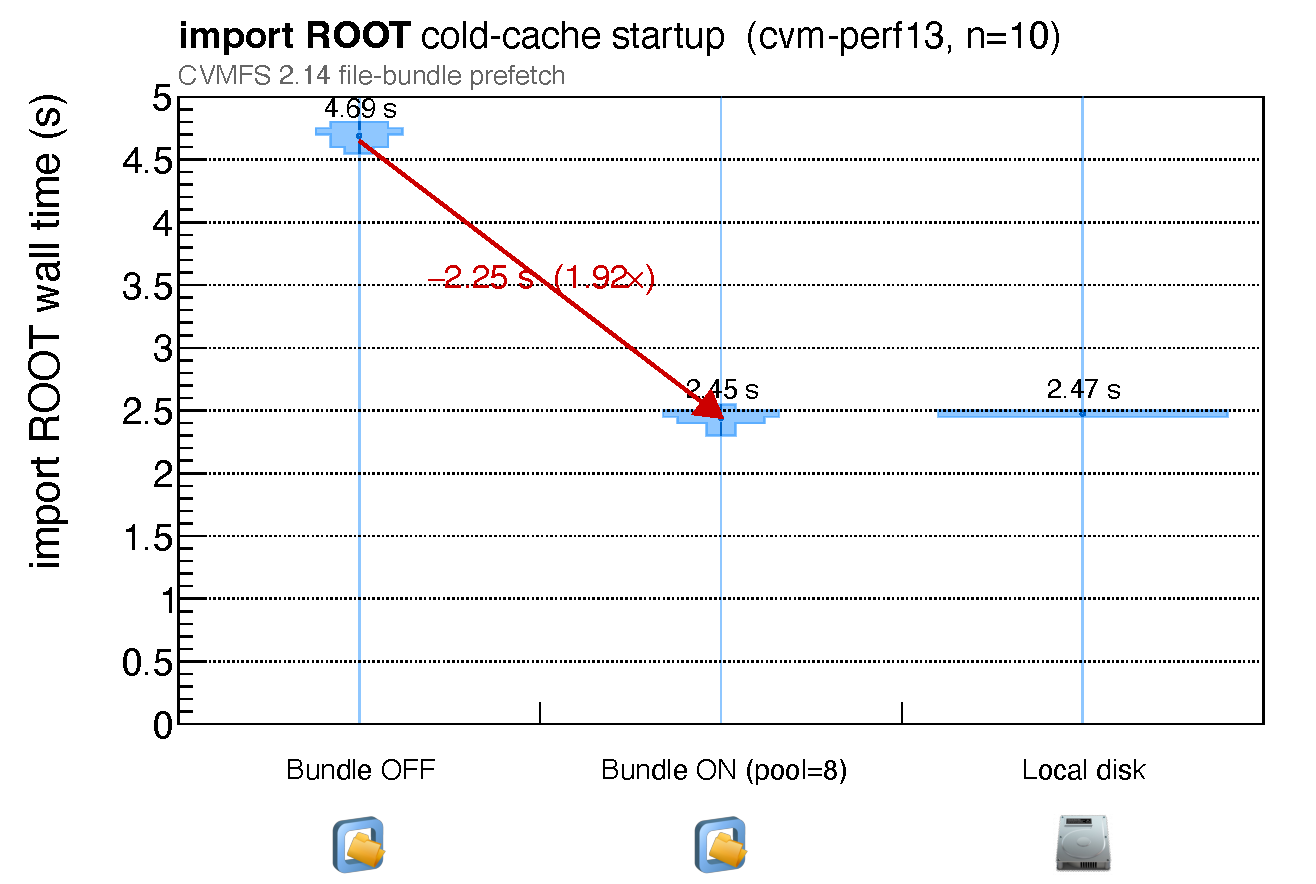
\includegraphics[width=0.62\textwidth]{figures/violin_bundle.pdf}
\caption{Distribution of ROOT startup times. With filebundles enabled
(\texttt{CVMFS\_PREFETCH\_FILEBUNDLES=ON}), CernVM-FS startup matches
local-disk performance, closing the gap to the on-demand cold-cache
baseline.}
\label{fig-violin}
\end{figure}

\subsection{Prefetch thread pool}
\label{sec-pool}

Prefetching is implemented with a pool of worker threads whose size is
set by \texttt{CVMFS\_BUNDLE\_POOL\_SIZE}. As shown in
Fig.~\ref{fig-pool}, startup performance improves as workers are added
but saturates around eight threads, which is also the default. Most of
the benefit is therefore obtained with a moderate amount of concurrency
and without aggressive tuning.

\begin{figure}[t]
\centering
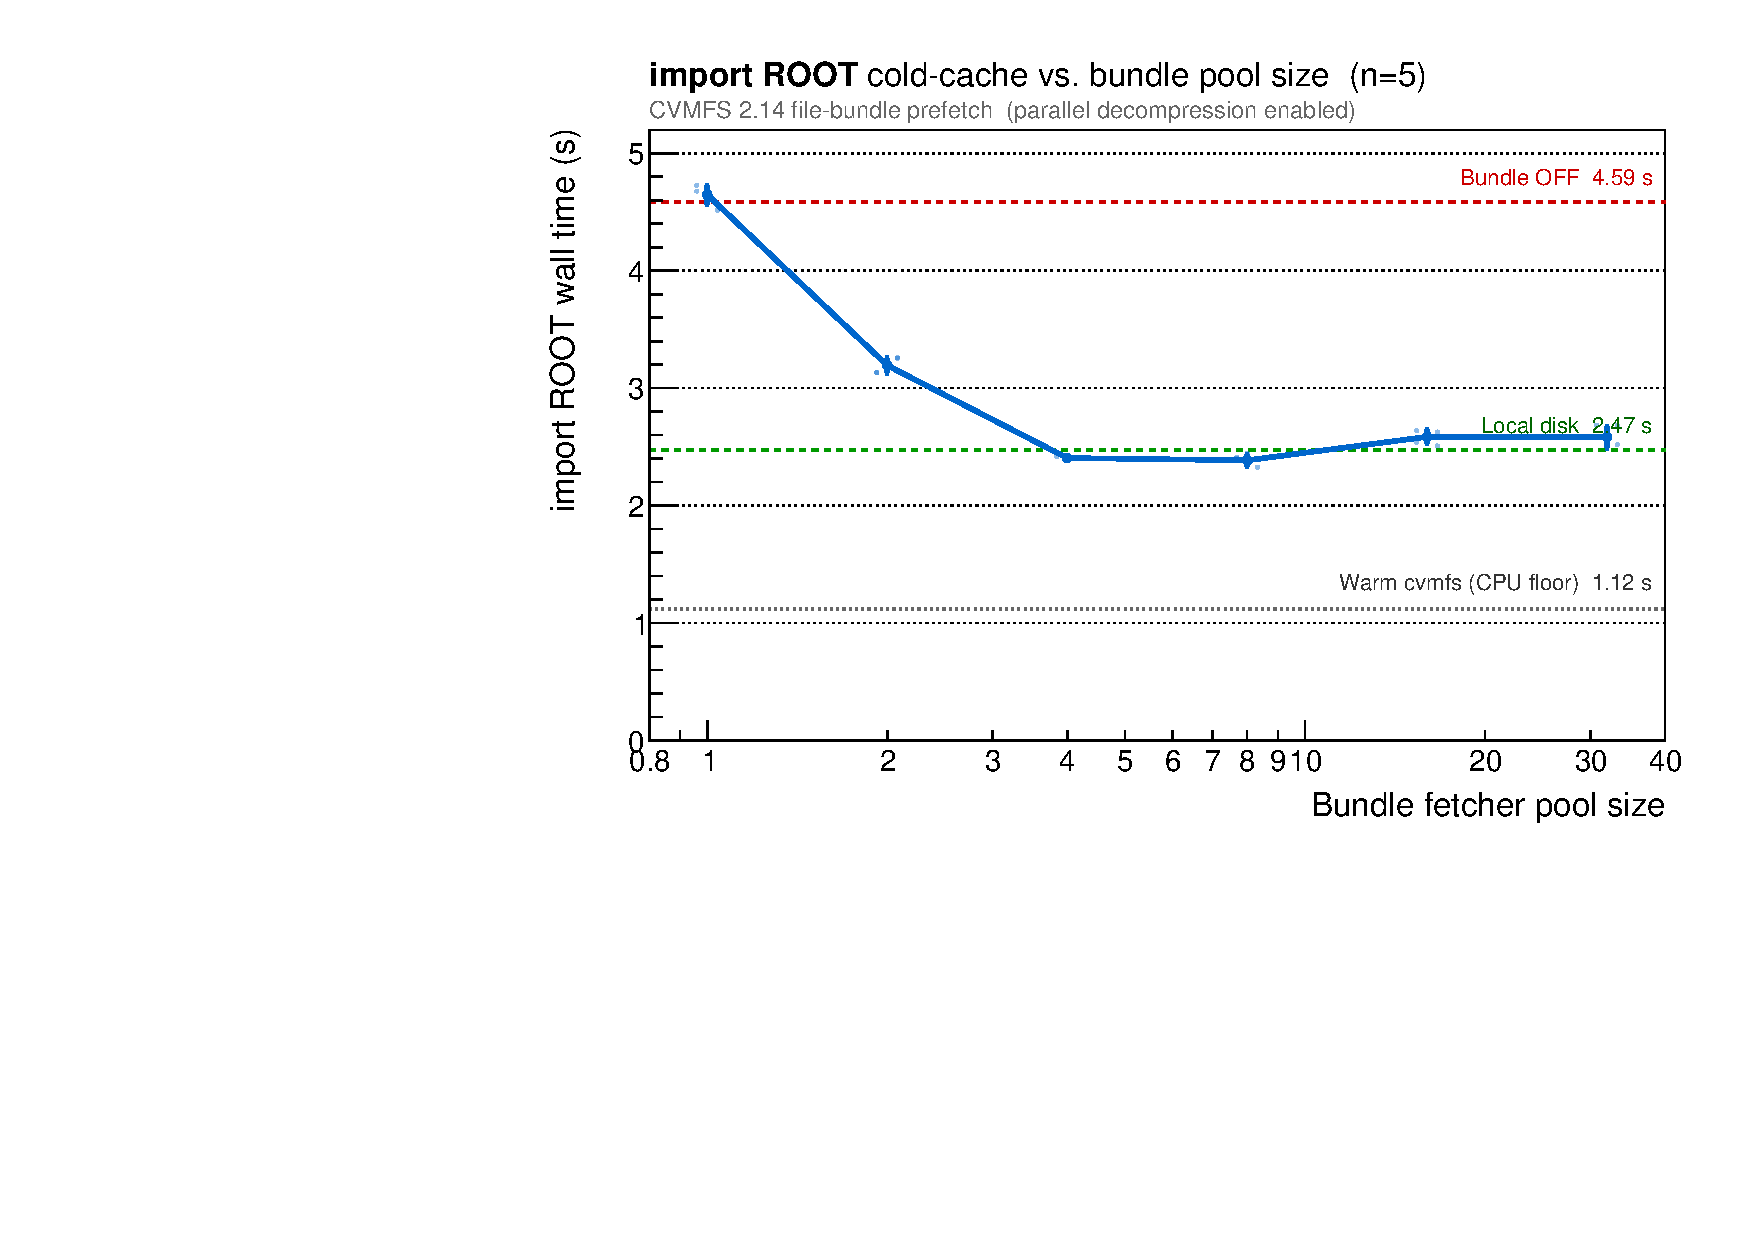
\includegraphics[width=0.62\textwidth]{figures/pool_scan.pdf}
\caption{ROOT startup time as a function of the prefetch thread-pool
size (\texttt{CVMFS\_BUNDLE\_POOL\_SIZE}). Performance saturates around
eight worker threads, the default.}
\label{fig-pool}
\end{figure}

\subsection{Network latency}
\label{sec-latency}

The benefit is most pronounced under network latency. We artificially
injected loopback round-trip latency using \texttt{tc qdisc netem}.
Without filebundles, startup time grows roughly linearly with the
round-trip time, because the application must wait for many small
dependent fetches in sequence. With filebundles enabled, startup time
stays nearly flat over a substantial range (Fig.~\ref{fig-latency}),
because the requests are prefetched concurrently: in this idealized
case the round-trip penalty is paid only for a small number of batches
rather than once per file.

\begin{figure}[t]
\centering
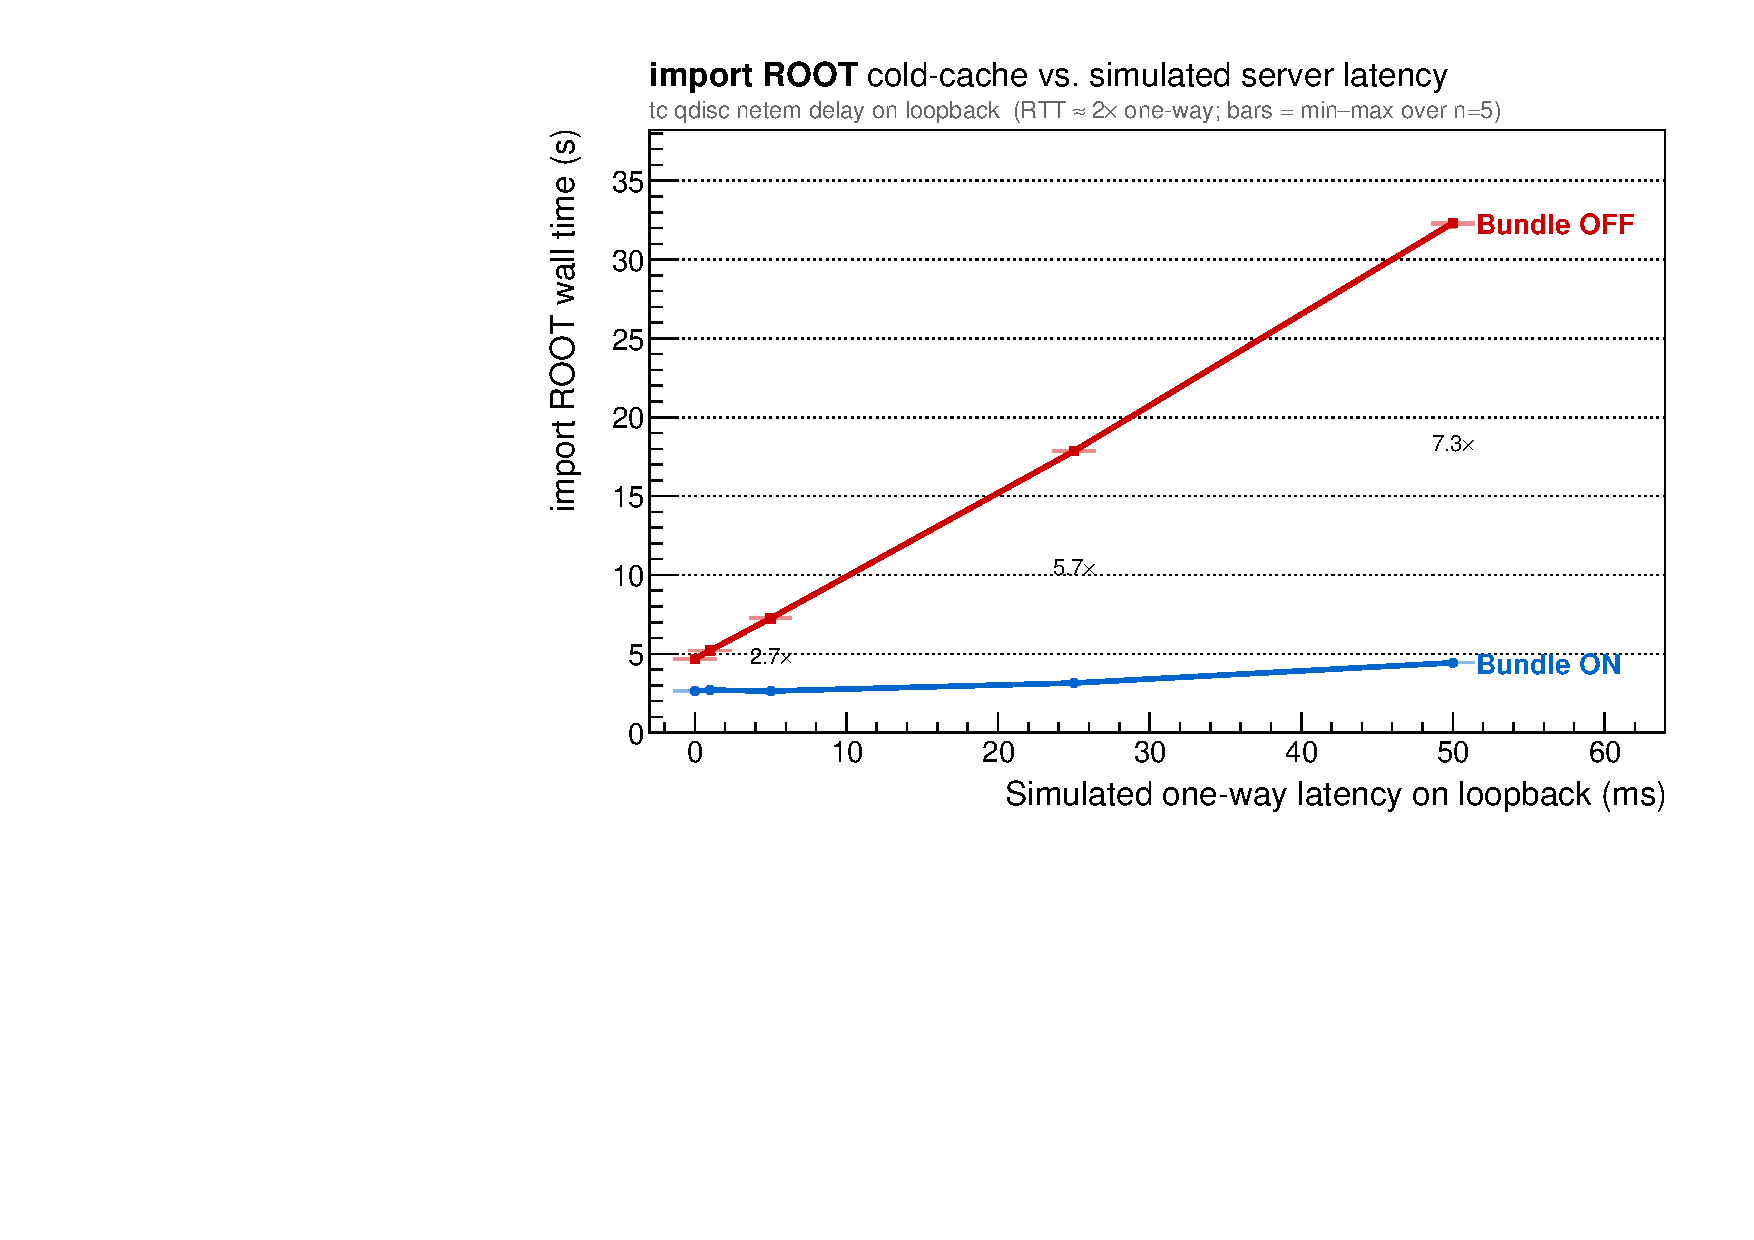
\includegraphics[width=0.62\textwidth]{figures/latency_scan.pdf}
\caption{ROOT startup time as a function of injected round-trip
latency. The on-demand baseline degrades roughly linearly, while
filebundles keep startup nearly flat by overlapping requests.}
\label{fig-latency}
\end{figure}

\subsection{Caveats}
\label{sec-caveats}

Filebundles do not reduce the total amount of data transferred; they
compress the startup traffic into a short, intense burst. In the
benchmark, requests peak at about 1480~per~second with filebundles,
versus about 680~per~second without them (Fig.~\ref{fig-burst}). The
feature should therefore be used selectively, in particular on
interactive systems such as \texttt{lxplus}, where startup latency
matters most. Over-prefetching should be avoided, and any rollout
should be coordinated with proxy and site administrators so that the
request bursts do not overload shared caches.

\begin{figure}[t]
\centering
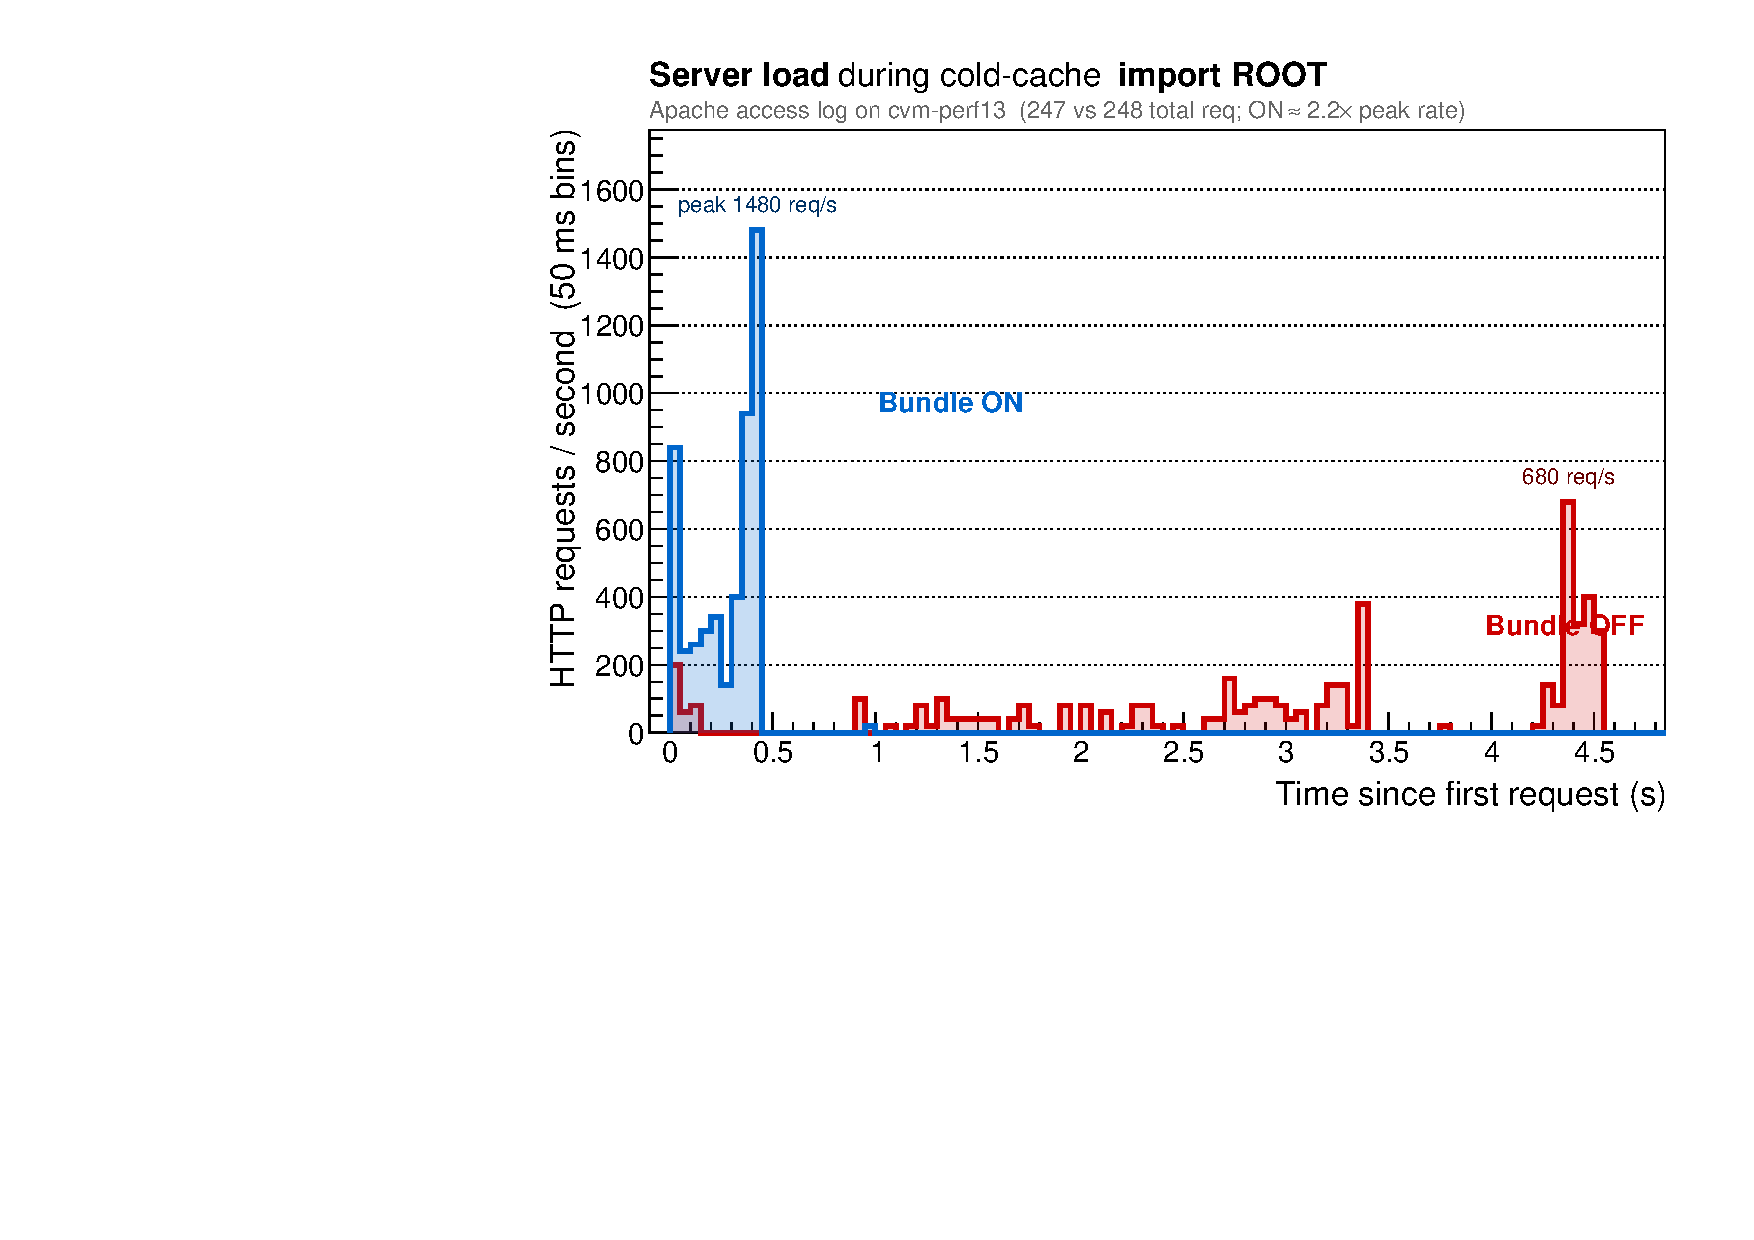
\includegraphics[width=0.62\textwidth]{figures/req_burst.pdf}
\caption{Request rate during startup. Filebundles concentrate the same
total traffic into a shorter, more intense burst (peak ${\sim}1480$
req/s versus ${\sim}680$ req/s without bundles).}
\label{fig-burst}
\end{figure}

%======================================================================
\section{Outlook}
\label{sec-outlook}

Several directions for future work remain. FUSE passthrough, available
in CernVM-FS 2.14 on newer kernels, allows direct kernel I/O on cached
objects after \texttt{open()} and should reduce overhead further;
proper benchmarks combining it with filebundles are still needed. For
CernVM-FS 2.15 we plan better tooling for filebundle creation, with
more automation, more robust updates, and support for specifying file
chunks in bundle specifications. Finally, we are considering packfiles
that aggregate many small objects in backend storage to reduce request
overhead at the source; the main challenge there is backward
compatibility.

%======================================================================
\section{Conclusions}
\label{sec-conclusions}

CernVM-FS filebundles are an effective way to accelerate application
startup when many files are needed immediately. They require some
effort from the librarian -- tracing startup behaviour and publishing a
\texttt{.cvmfsbundle} specification next to a trigger file -- but in
return they can dramatically reduce cold-start latency, match local-disk
startup performance, and remain robust as network latency grows where
the on-demand baseline degrades linearly. The feature is available in
CernVM-FS 2.14 and is enabled per mount with
\texttt{CVMFS\_PREFETCH\_FILEBUNDLES}. Used selectively on interactive
systems, it closes much of the gap between a globally distributed,
on-demand file system and local disk.

\vspace{0.5em}
\noindent\textbf{Acknowledgements.} We thank Chris Burr (LHCb) for the
input that motivated this work, and the CernVM-FS team at CERN.

\vspace{0.3em}
\noindent\emph{Disclosure: AI-based tools were used to assist with
drafting and formatting this manuscript; all content was reviewed and
verified by the authors.}

%======================================================================
\begin{thebibliography}{9}

\bibitem{ref-cvmfs}
J. Blomer, P. Buncic, R. Meusel, G. Ganis, I. Sfiligoi, D. Thain,
The need for a versioned data analysis software environment,
in \textit{Proc.\ of the 9th IEEE International Conference on
e-Science} (2013).
\url{https://doi.org/10.1109/eScience.2013.44}

\bibitem{ref-cvmfs-tech}
J. Blomer, C. Aguado-S\'anchez, P. Buncic, A. Harutyunyan,
Distributing LHC application software and conditions databases using
the CernVM file system, J.\ Phys.: Conf.\ Ser.\ \textbf{331}, 042003
(2011). \url{https://doi.org/10.1088/1742-6596/331/4/042003}

\bibitem{ref-docs}
CernVM-FS documentation.
\url{https://cvmfs.readthedocs.io/}

\end{thebibliography}

\end{document}
